\begin{frame}
	\frametitle{День 11. 28 августа}
	\framesubtitle{д.р. Чиринкол~--- д.р. Кубань} % Optional subtitle
	\begin{columns}[c] % The "c" option specifies centered vertical alignment while the "t" option is used for top vertical alignment
		\begin{column}{0.55\textwidth} % Left column width
			\begin{itemize}
				\item Четверо сходят
				\item Солнышко светит
				\item Лёша психанул
				\item Прошли \textbf{12.7} км
				\item ЧХВ: 3:23
				\item Набор/сброс: \textcolor{darkred}{\textbf{+90}}/\textcolor{darkblue}{\textbf{-500}}~м
			\end{itemize}			
		\end{column}
		\begin{column}{0.45\textwidth} % Right column width
			\centering
			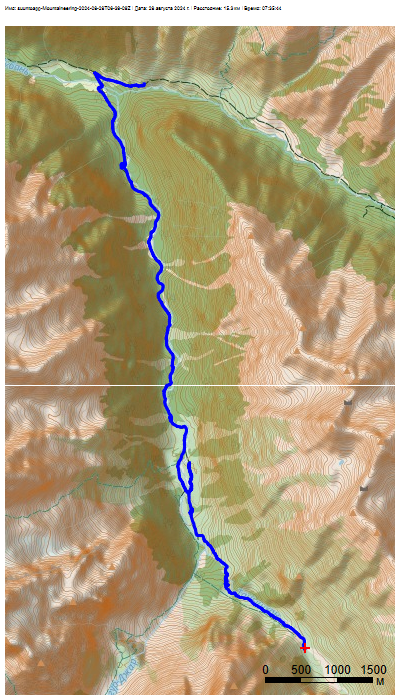
\includegraphics[width=\linewidth]{../pics/mini_maps/28}
		\end{column}
	\end{columns}
\end{frame}

\begin{frame}
	\frametitle{Настроение руководителя}
	\framesubtitle{День 11, 28 августа}	
	\centering
	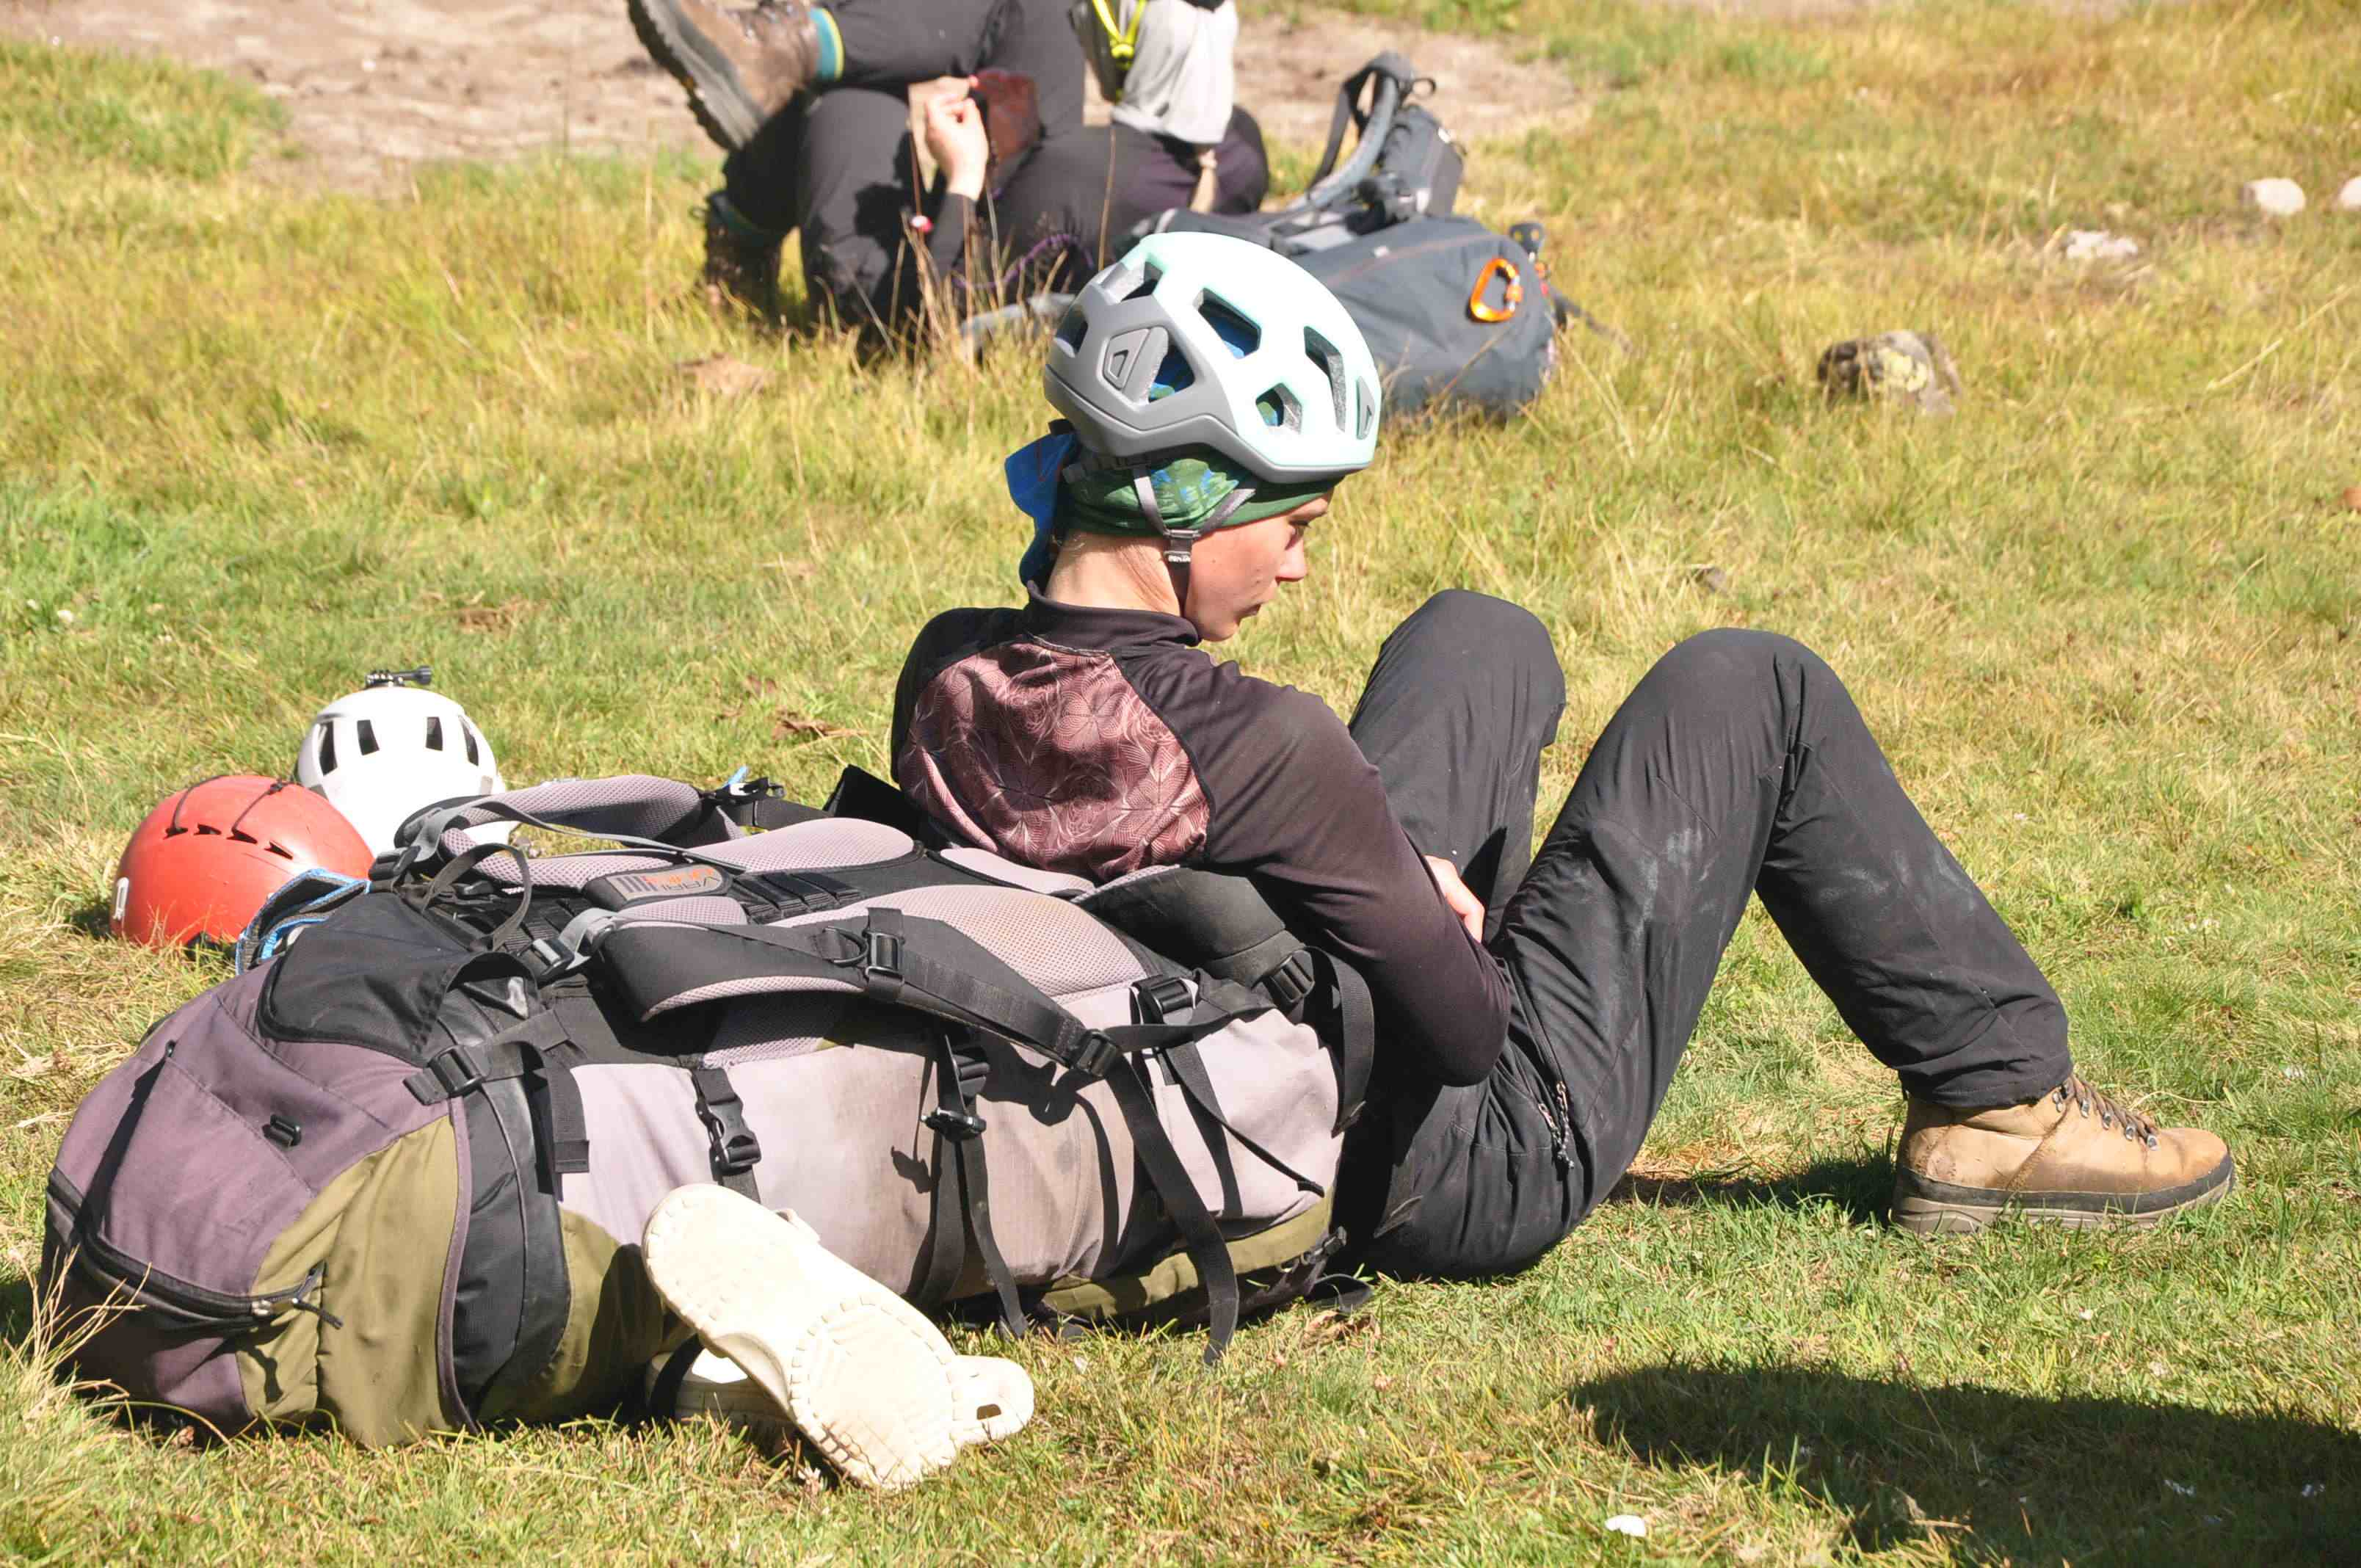
\includegraphics[width=\textwidth]{../pics/DSC_0435 2}			
\end{frame}

\begin{frame}
	\frametitle{Руководы}
	\framesubtitle{День 11, 28 августа}	
	\centering
	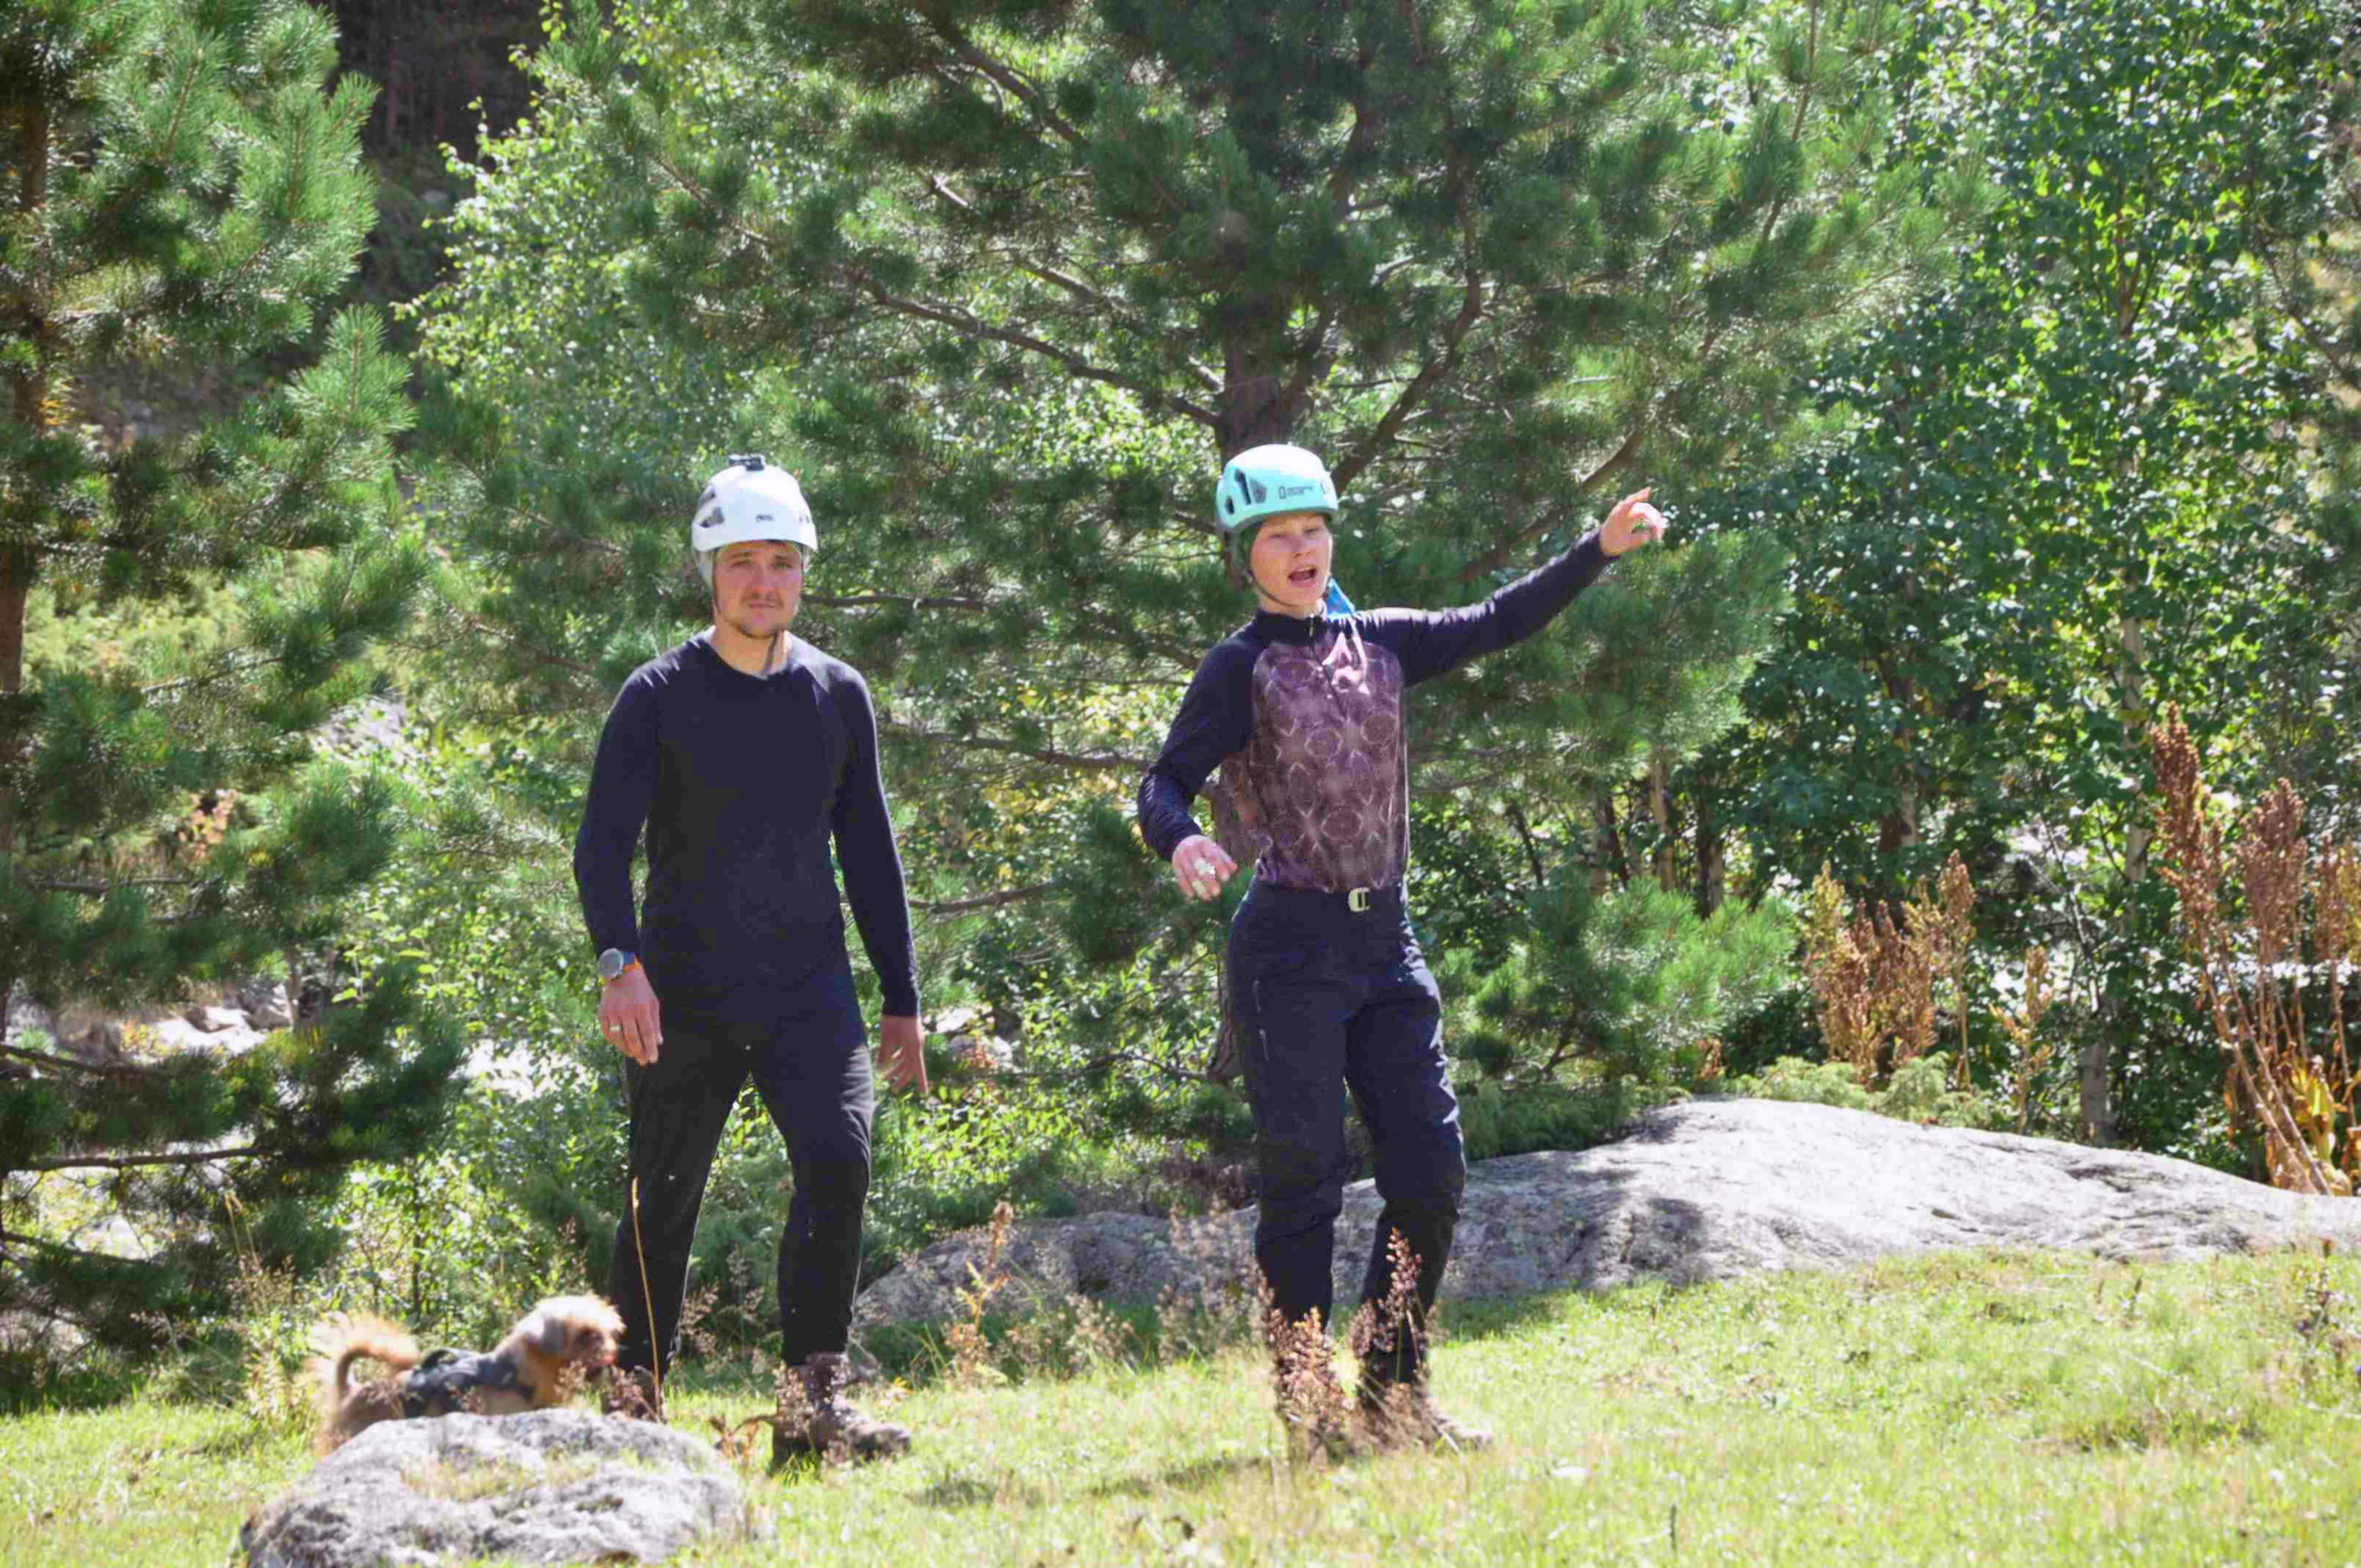
\includegraphics[width=\textwidth]{../pics/DSC_0455 2}			
\end{frame}

\begin{frame}
	\frametitle{Д.р. Чунгур-Джар}
	\framesubtitle{День 11, 28 августа}	
	\footnotesize Именно эти ступени мы обходили через пер. Перемётный
	\centering
	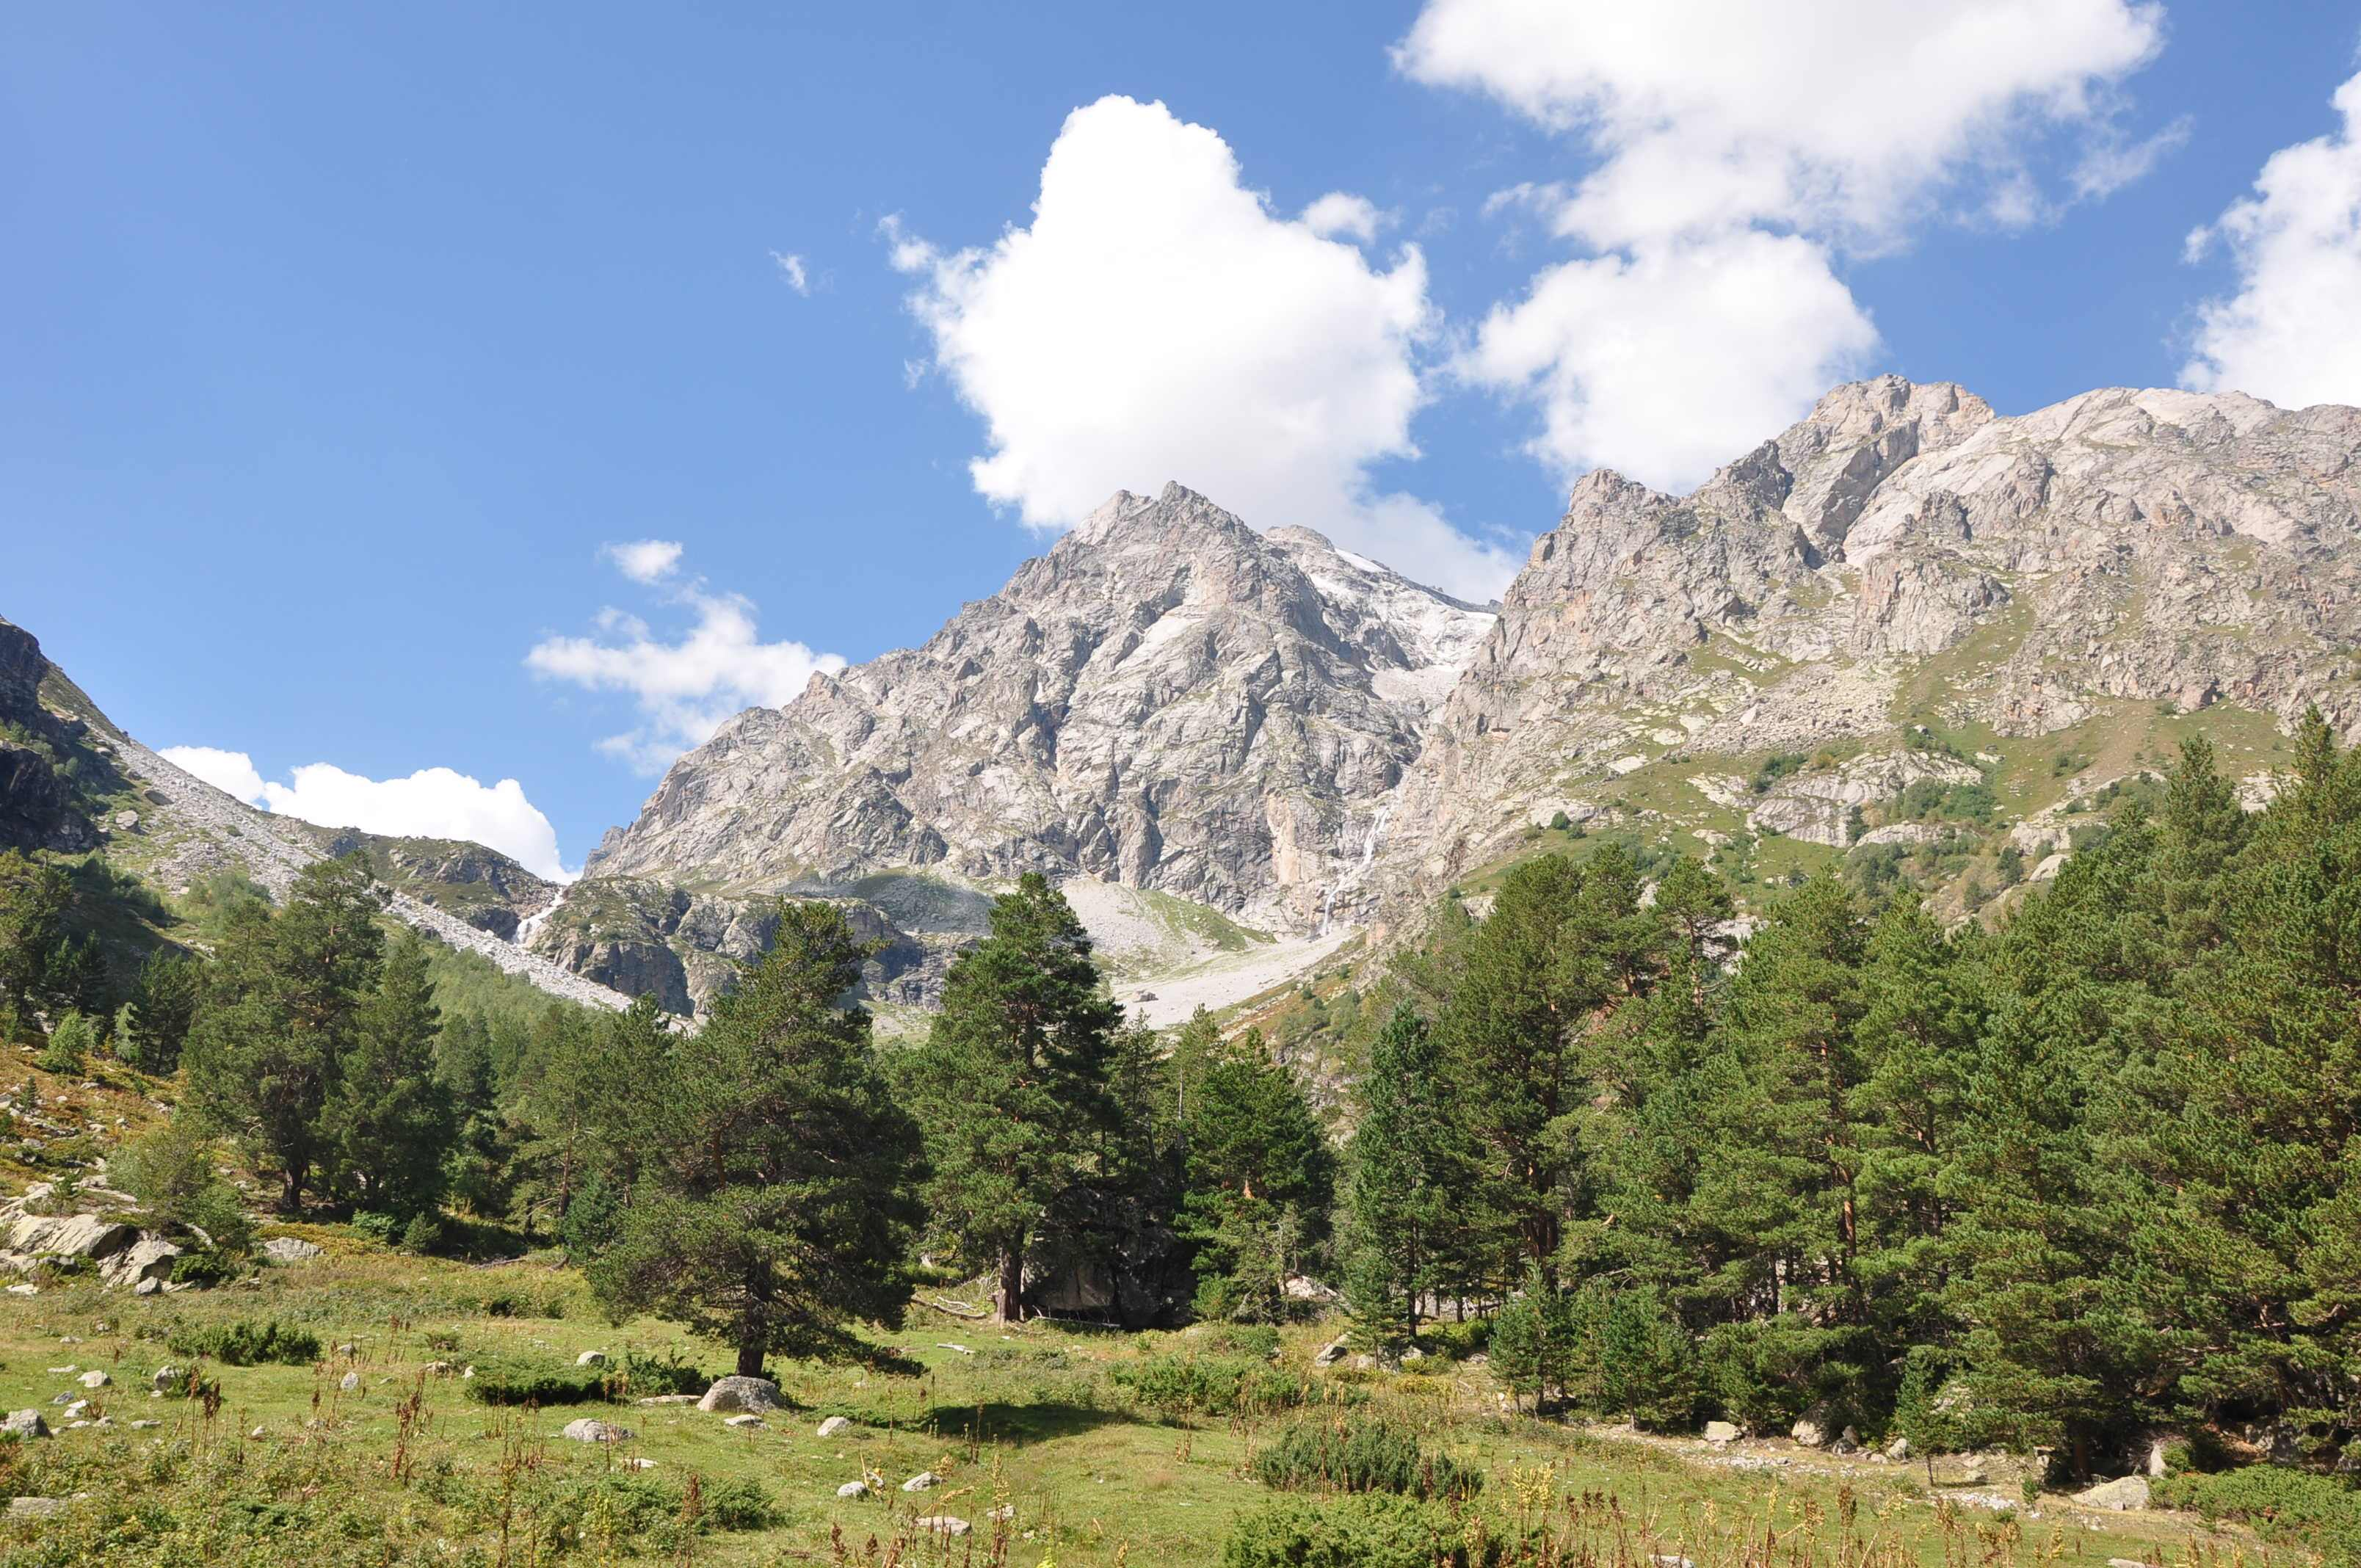
\includegraphics[width=0.95\textwidth]{../pics/DSC_0459 2}			
\end{frame}

\begin{frame}
	\frametitle{Вид д.р. Чиринкол}
	\framesubtitle{День 11, 28 августа}	
	\footnotesize«Чирин къол»~--- «Гнилое ущелье»
	\centering
	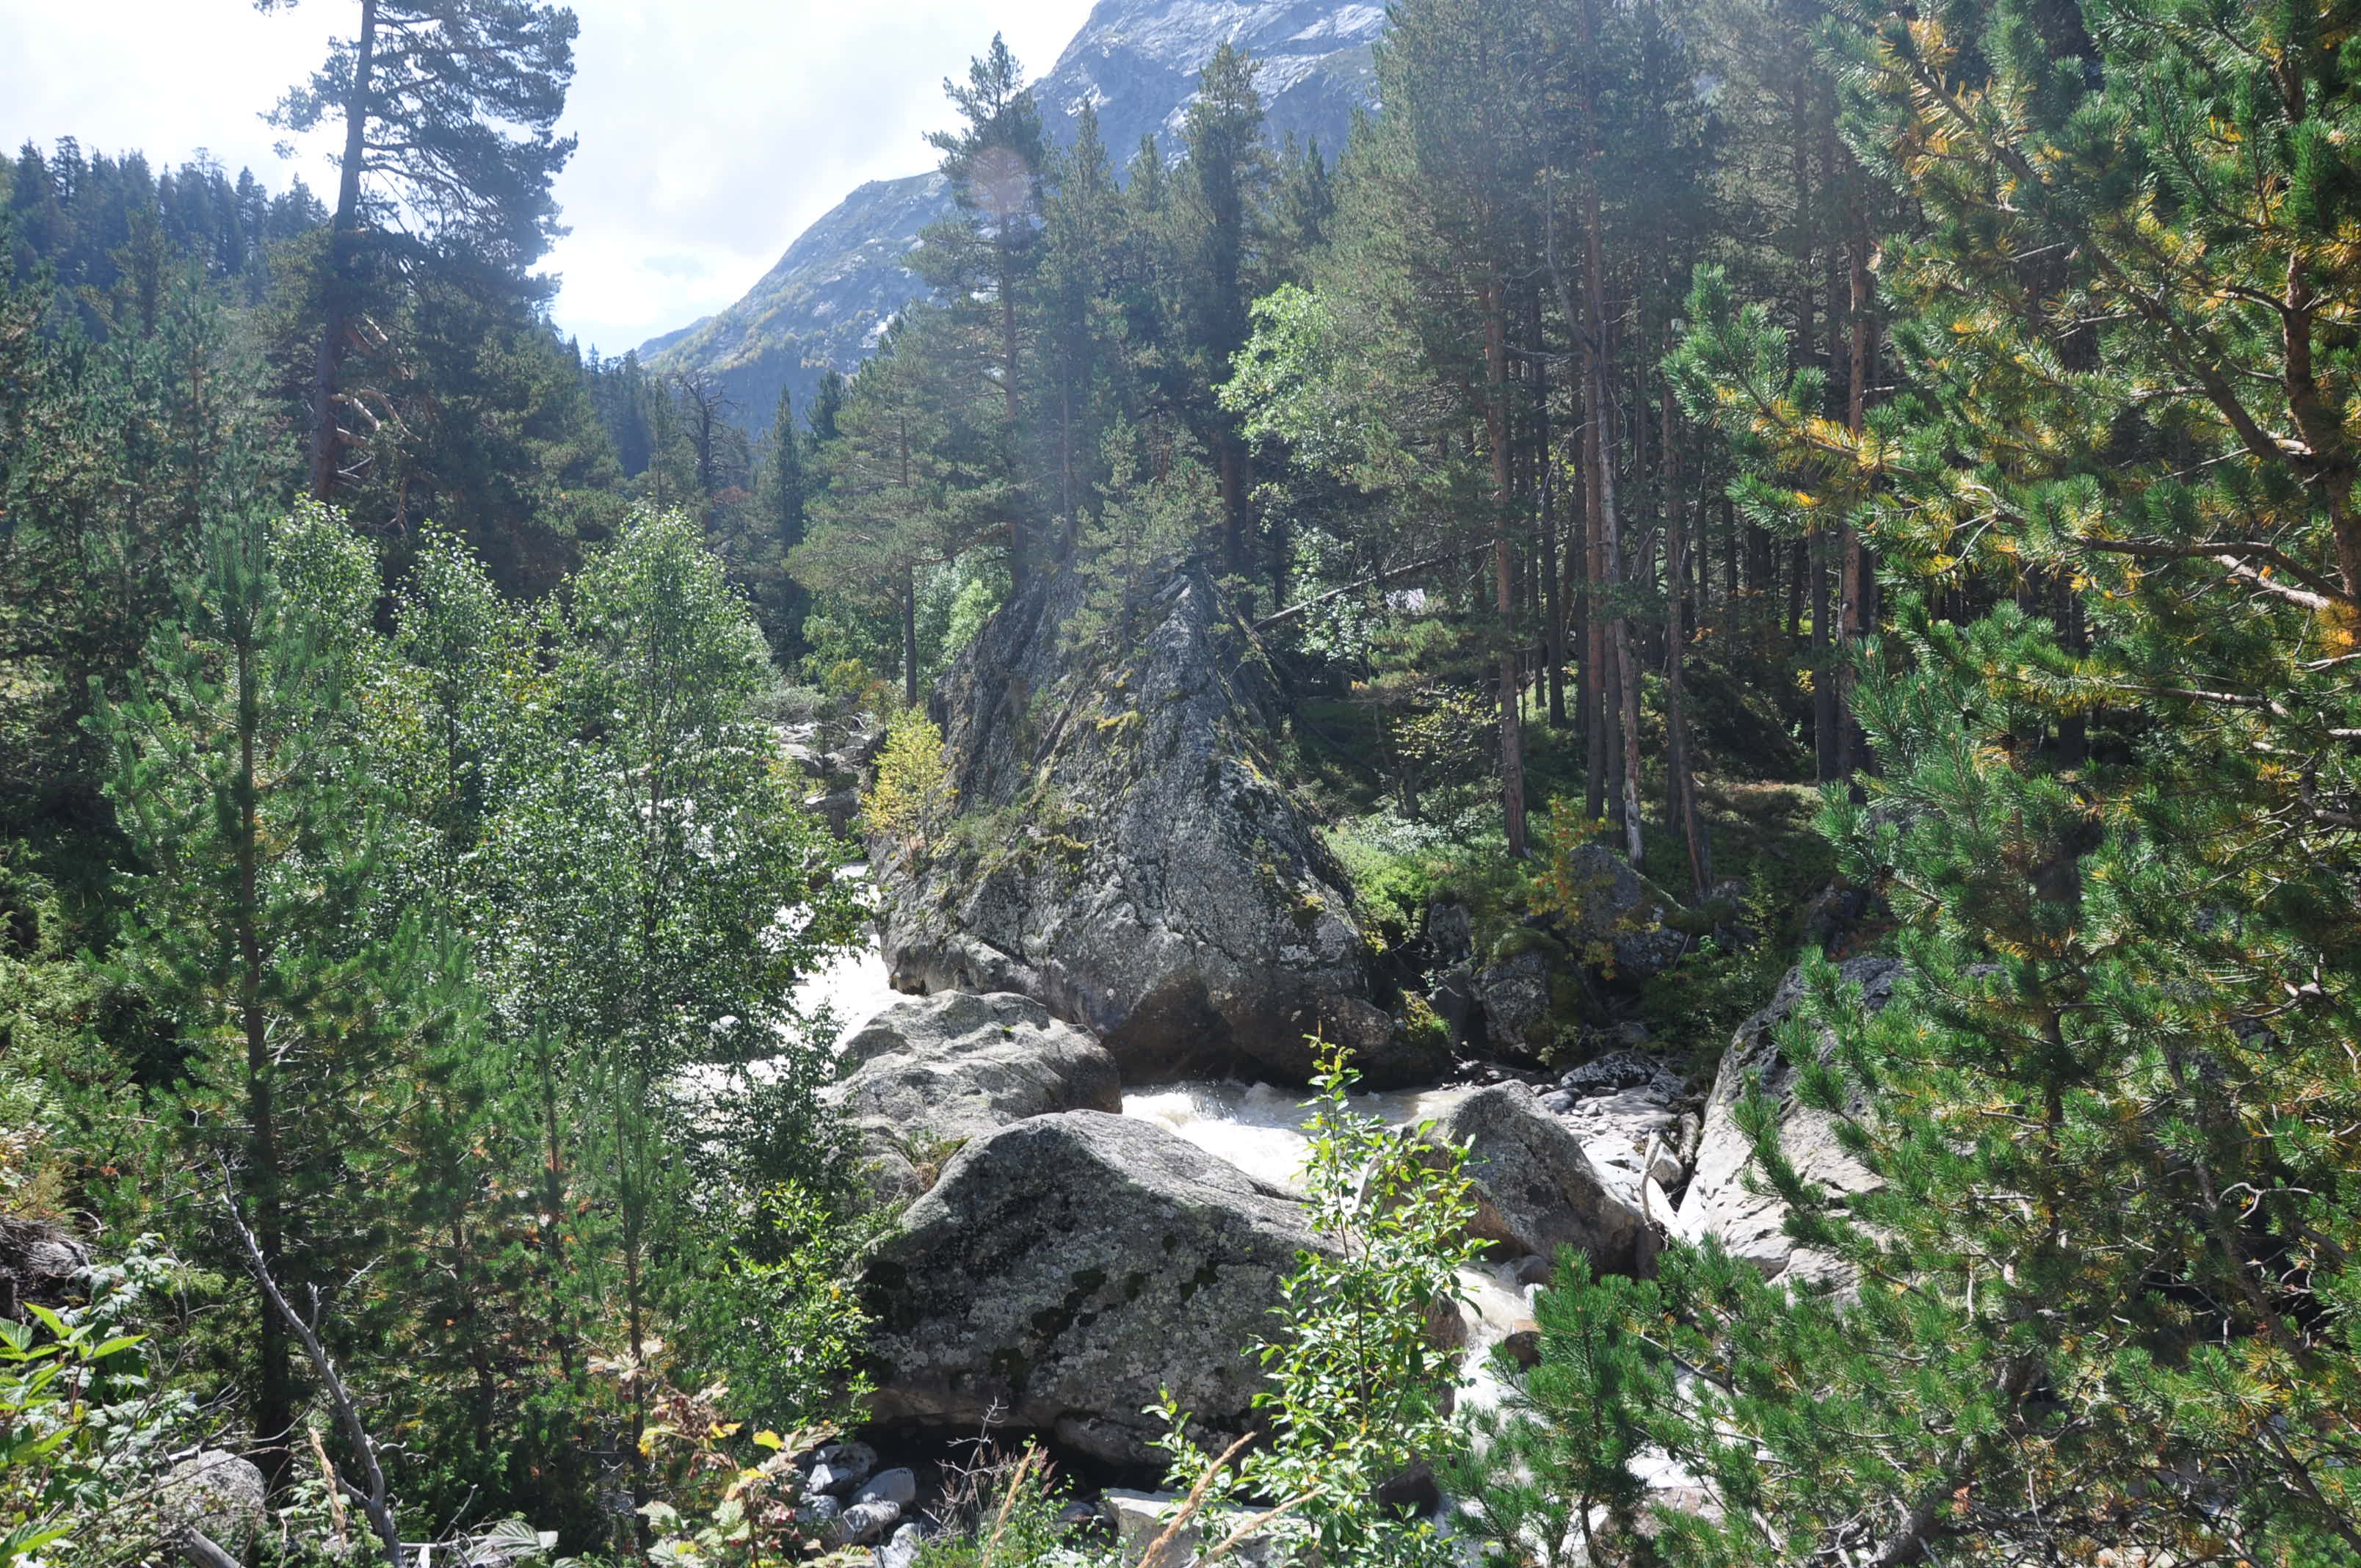
\includegraphics[width=0.9\textwidth]{../pics/DSC_0461 2}			
\end{frame}

\begin{frame}
	\frametitle{Вид д.р. Чиринкол}
	\framesubtitle{День 11, 28 августа}	
	\centering
	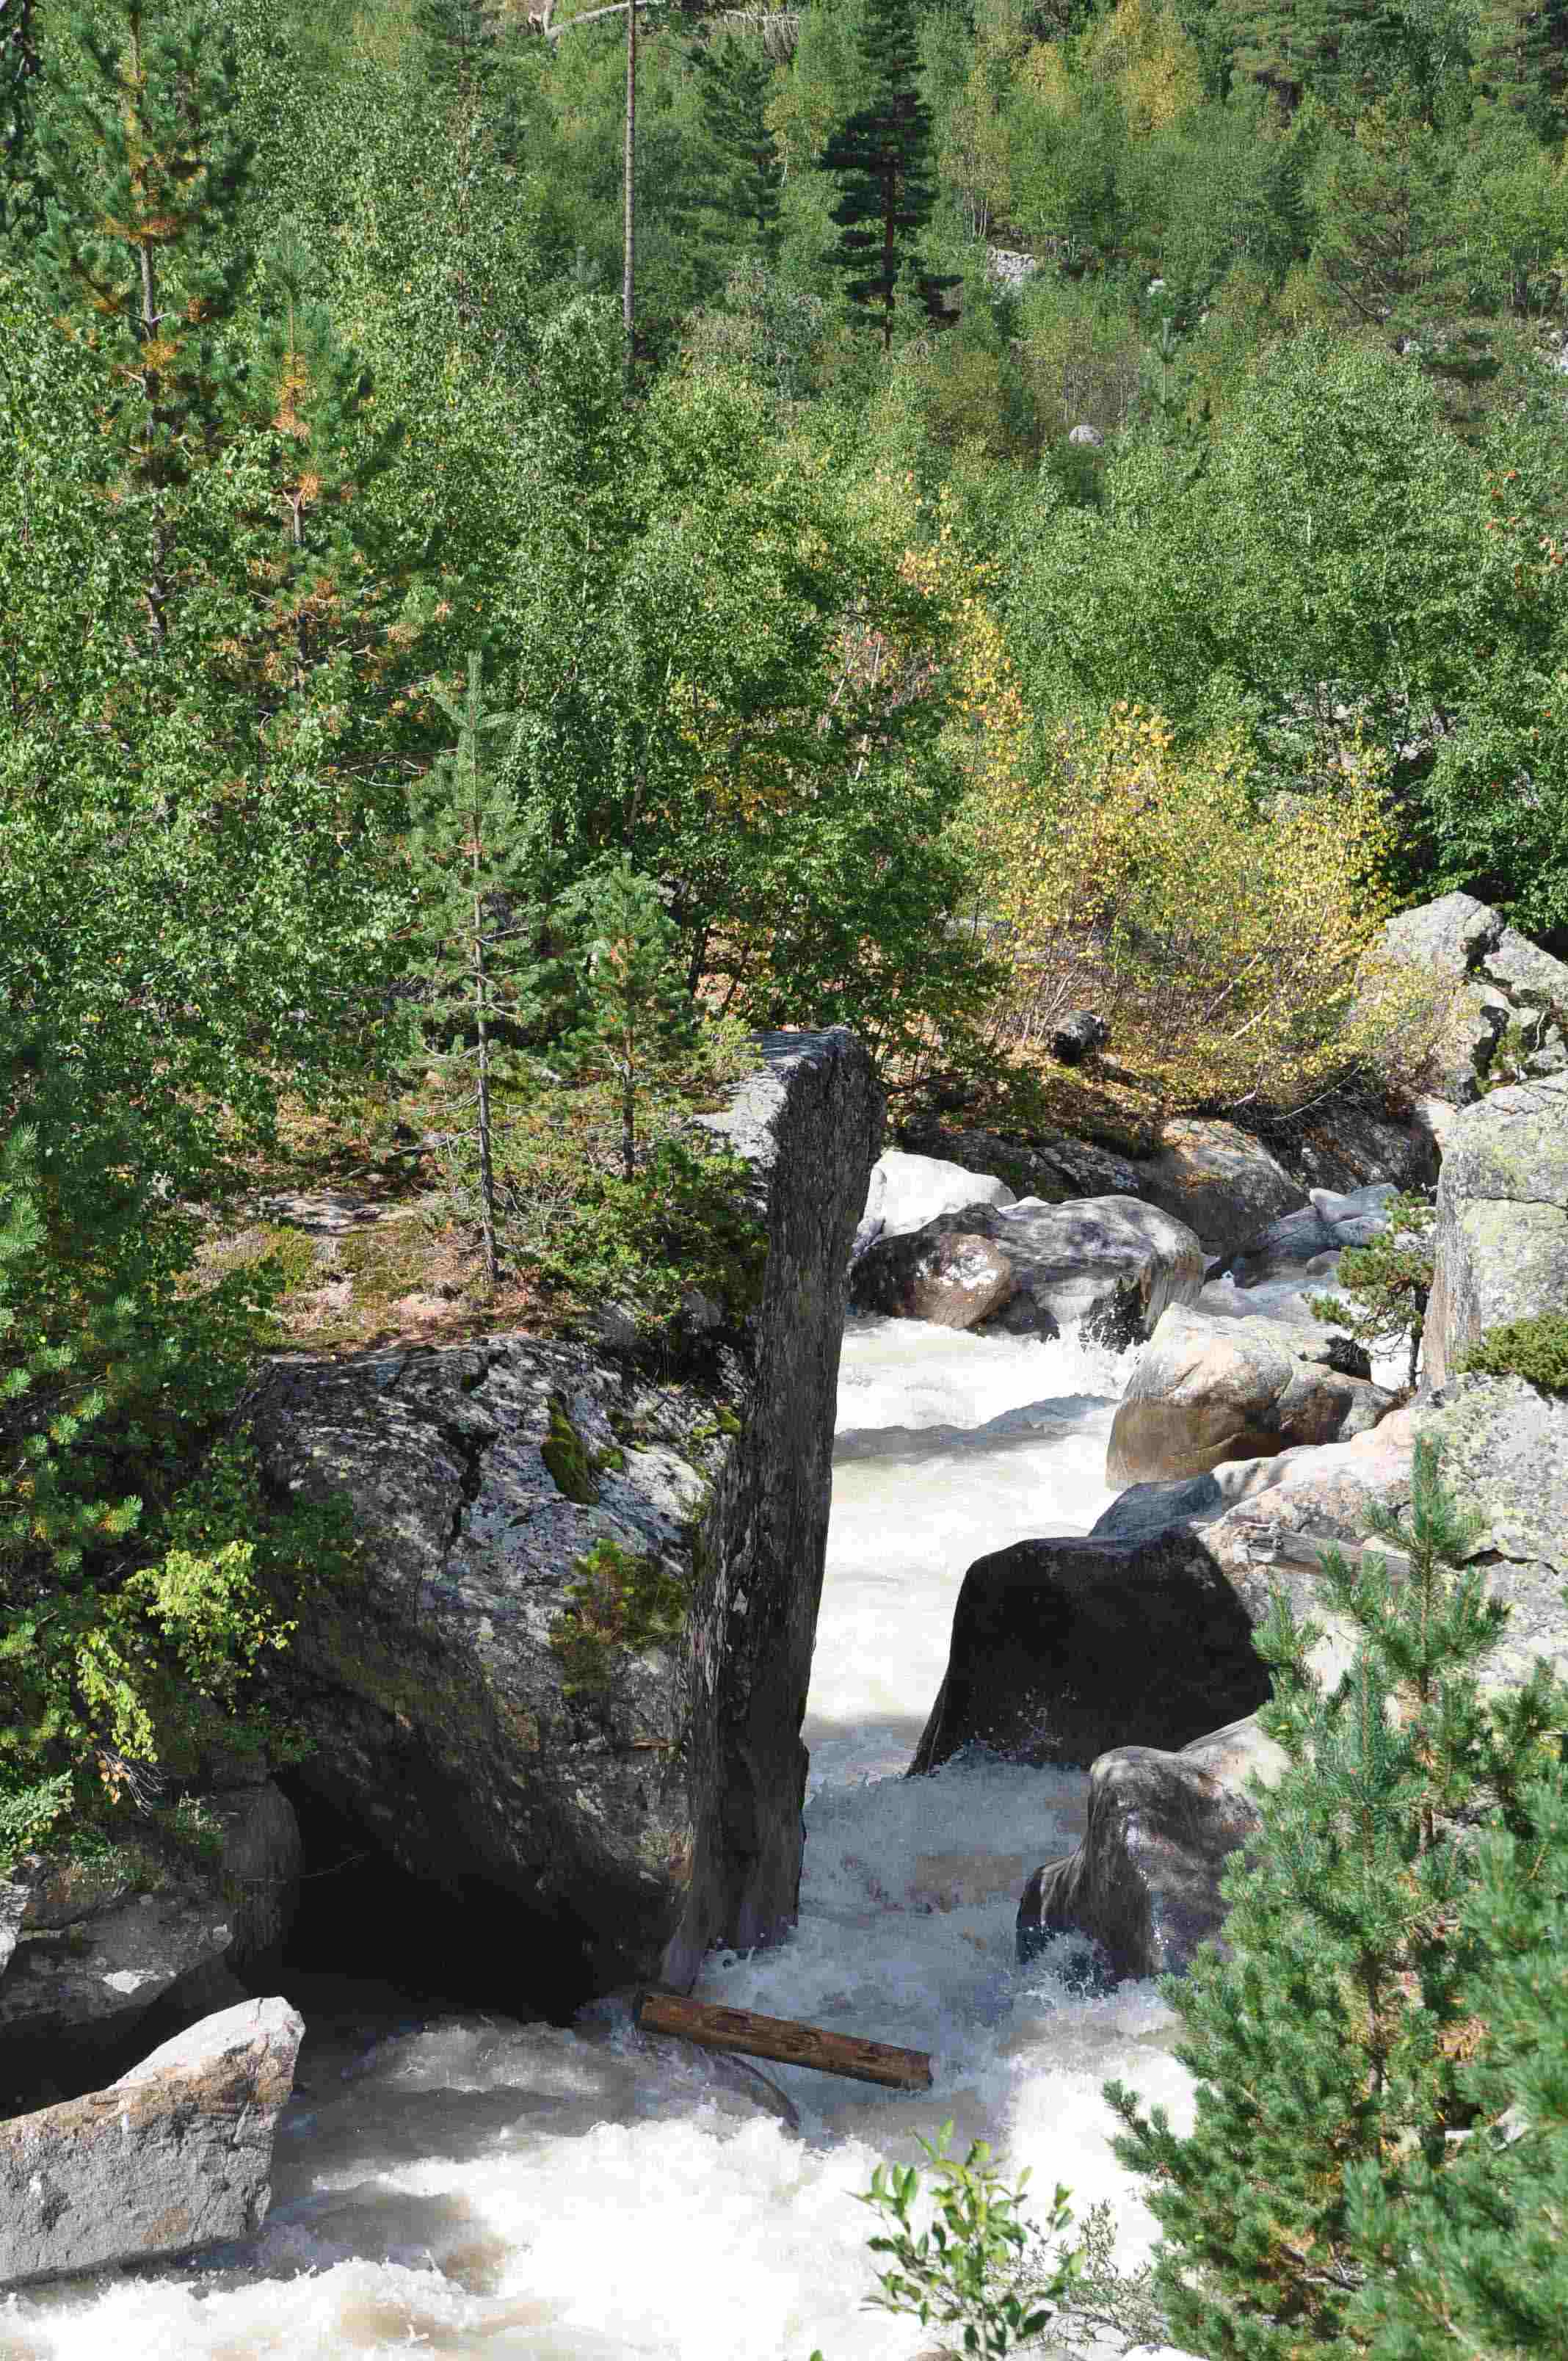
\includegraphics[width=0.45\textwidth]{../pics/DSC_0460 2}			
\end{frame}

\begin{frame}
	\frametitle{Вилка долин}
	\framesubtitle{День 11, 28 августа}	
	\centering
	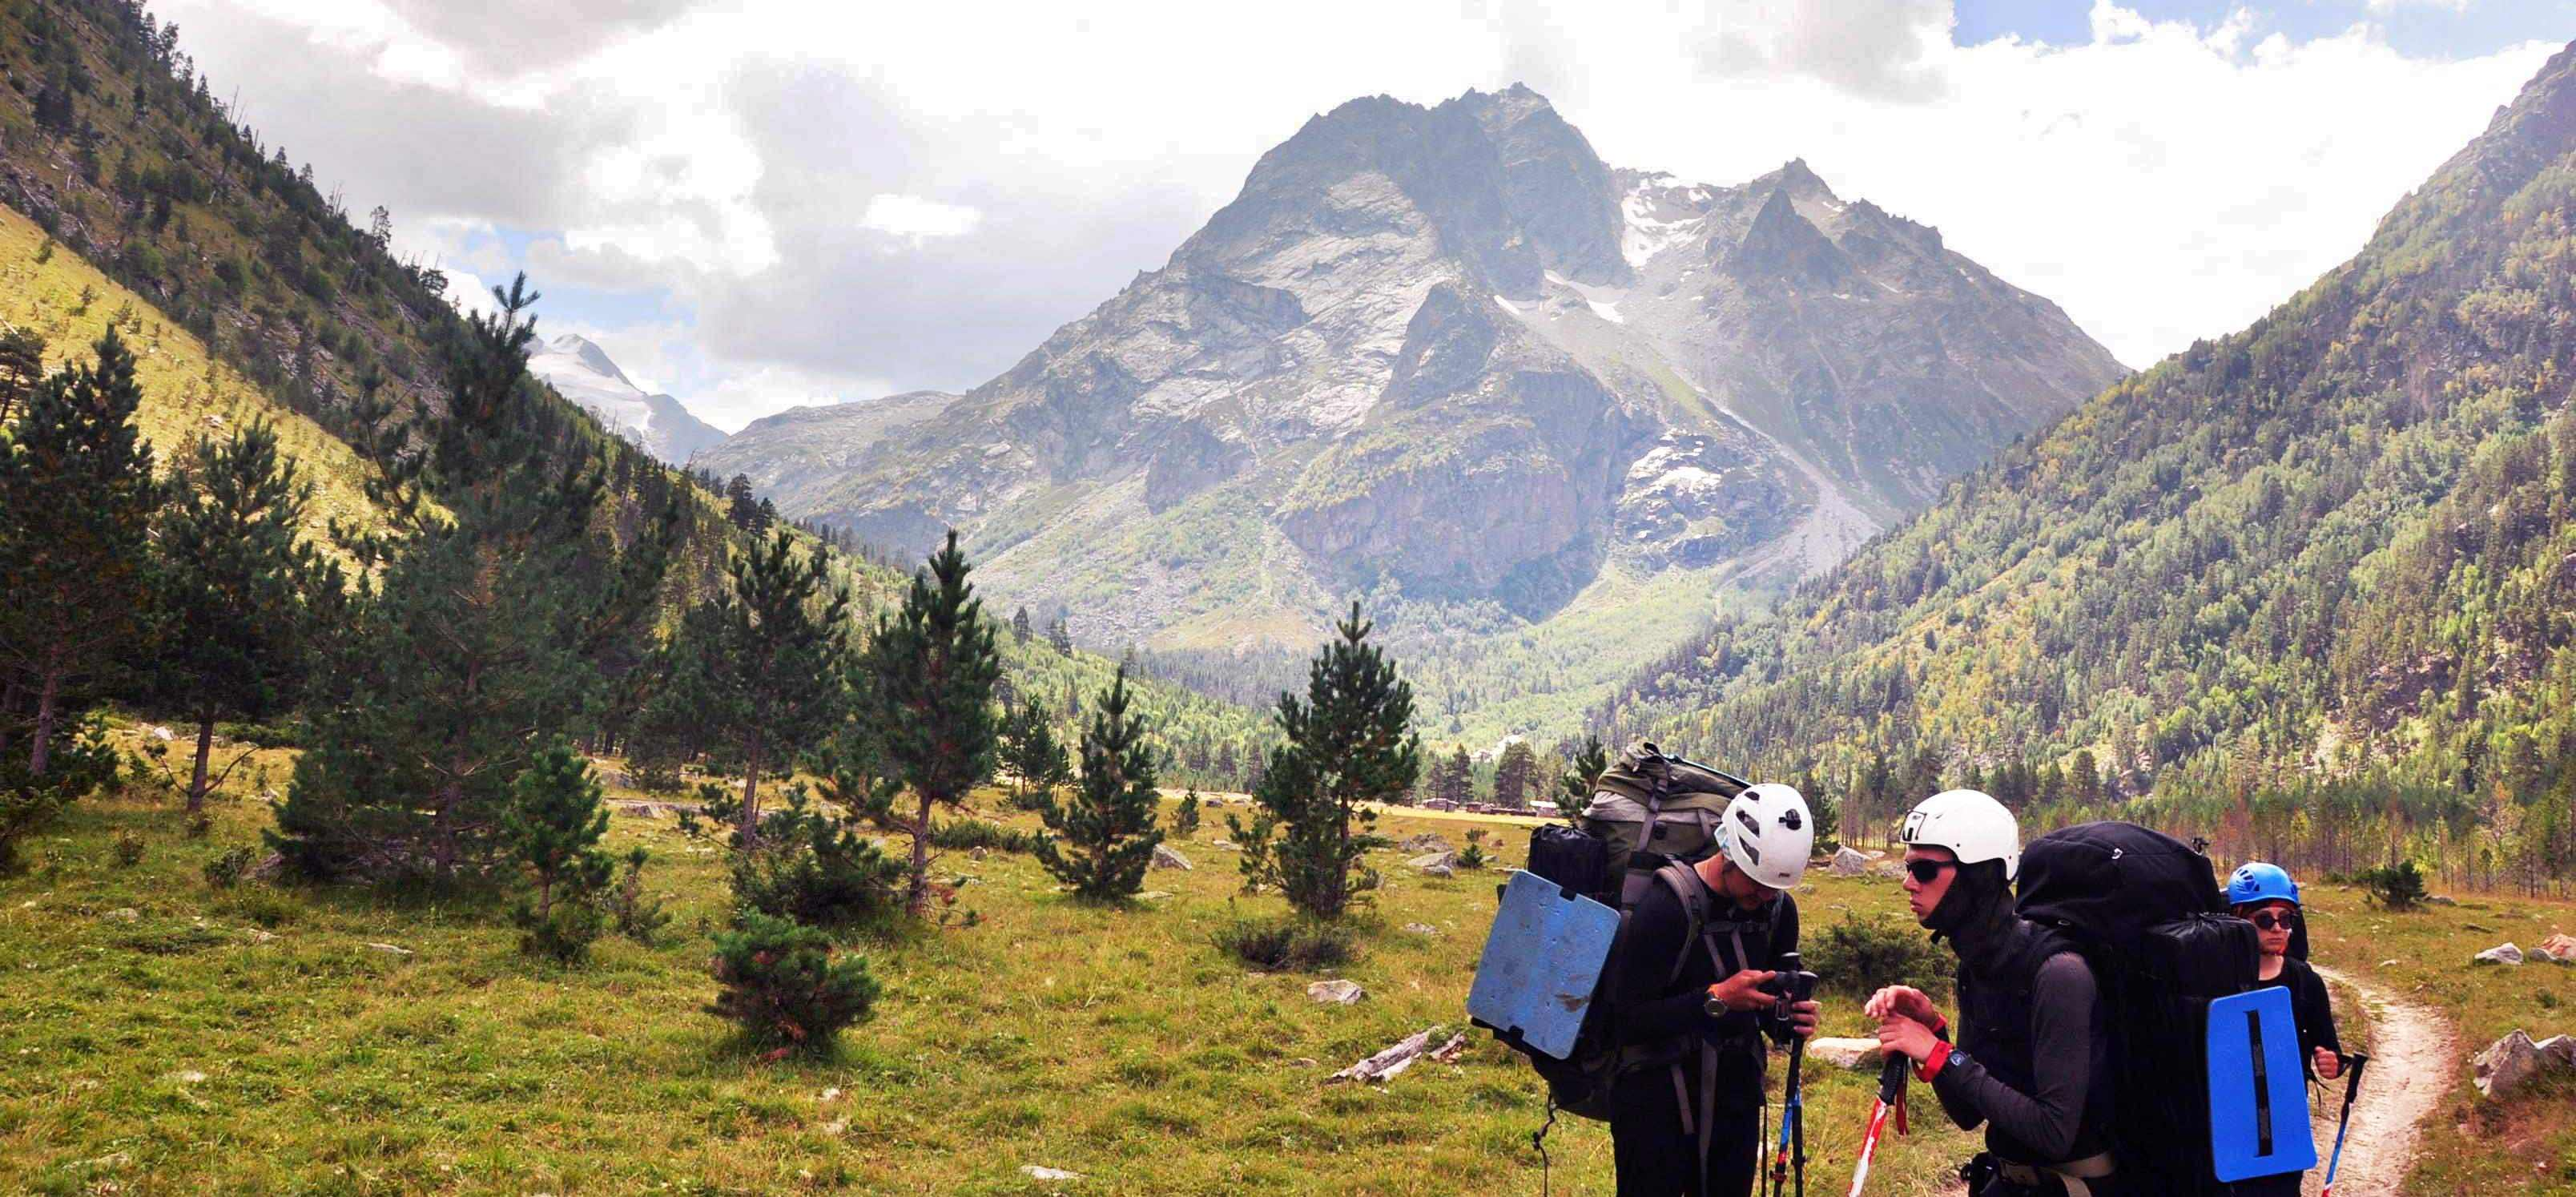
\includegraphics[width=\textwidth]{../pics/DSC_0462 2}			
\end{frame}
